% document class and packages
\documentclass{beamer}
\usepackage{adjustbox}
\usepackage{algorithm,algorithmic}
\usepackage{amsmath}
\usepackage{amssymb}
\usepackage{color, colortbl}
\usepackage{graphicx}
\usepackage{hyperref}
\usepackage{pgfplots}
\pgfplotsset{compat=1.14}
\usepackage{tikz}

% indent for algorithm pseudo-code
\newlength\myindent
\setlength\myindent{1em}
\newcommand\bindent{%
  \begingroup
  \setlength{\itemindent}{\myindent}
  \addtolength{\algorithmicindent}{\myindent}
}
\newcommand\eindent{\endgroup}

% new commands and math operators
\newcommand*\conj[1]{\overline{#1}}
\newcommand{\iu}{{i\mkern1mu}}
\newcommand\abs[1]{\left|#1\right|}
\newcommand\norm[1]{\left\Vert#1\right\Vert}
\newcommand\diag[1]{\operatorname{diag}\left(#1\right)}
\newcommand\re[1]{\operatorname{Re}\left(#1\right)}
\newcommand\sv[2]{\operatorname{sv}_{#1}(#2)}
\newcommand\hd[2]{\operatorname{hd}(#1,#2)}
\newcommand\md[2]{\operatorname{md}(#1,#2)}
\newcommand\func[1]{\operatorname{function}~[#1]}
\DeclareMathOperator{\specr}{specR}
\DeclareMathOperator{\edger}{edgeR}

% 
\newtheorem{proposition}[theorem]{Proposition}

% remove figure caption prefix
\setbeamertemplate{caption}{\raggedright\insertcaption\par}

% hyperlinks setup
\hypersetup{colorlinks,breaklinks,
	urlcolor=[rgb]{0,0.75,1},
	linkcolor=[rgb]{0.75,0.75,0.75}}

% empty navigation symbols
\beamertemplatenavigationsymbolsempty

% remove navigation dots on miniframes
\makeatletter
\def\beamer@writeslidentry{\clearpage\beamer@notesactions}
\makeatother

% Use Theme
\usetheme{Warsaw}
\useoutertheme[footline=authortitle]{miniframes}
\useinnertheme[shadow=true]{rounded}

% Colors
\definecolor{black}{RGB}{0, 0, 0} % (primary, black)
\definecolor{lblue}{RGB}{102, 178, 255} % (secondary, light blue)
\definecolor{lgreen}{RGB}{102, 255, 178} %(tertiary, light green)
\definecolor{lsilver}{RGB}{224,224,224} % (text, light silver)
\definecolor{gray}{RGB}{128,128,128} % (graph node shade, gray)
\definecolor{white}{RGB}{255,255,255} % (graph node text, white)

% Beamer Colors
\setbeamercolor{palette primary}{bg=black,fg=lsilver}
\setbeamercolor{palette secondary}{bg=lblue,fg=lsilver}
\setbeamercolor{palette tertiary}{bg=black,fg=lsilver}
\setbeamercolor{structure}{fg=black} % itemize, enumerate, etc
\setbeamercolor{frametitle}{fg=black}

% Transparency for itemized listing
%\setbeamercovered{transparent}

% Title Page
\title{Rankability Updates}
\author{Thomas R. Cameron}
\institute{Davidson College}
\date{June 25, 2019}

\begin{document}
% Title Frame
\begin{frame}
	\titlepage
\end{frame}

% Outline
%\AtBeginSection[]{
 %\frame<beamer>{
  %\frametitle{Outline}   
  %\tableofcontents[currentsection]
 %}
%}

%%%%%%%%%%%%%%%%%%%%%%%%%%%%%%%%%%%%%%%%%%%%%%%%%%%%%%
%								SpecR Algorithm
%%%%%%%%%%%%%%%%%%%%%%%%%%%%%%%%%%%%%%%%%%%%%%%%%%%%%%
\section{SpecR Algorithm}

\begin{frame}{Update}
\begin{itemize}
\item	Spectral-degree characterization of \emph{complete dominance} graphs holds for all digraphs with weights $w_{ij}\in[0,1]$.
\vfill
\item	Therefore, we can model multiple games and tie situations and compare against the ideal complete dominance graph.
\end{itemize}
\end{frame}

\begin{frame}{Perturbation Theory}
\begin{itemize}
\item	The eigenvalues of the graph Laplacian of a complete dominance graph are extremely well-conditioned.
\vfill
\item	Therefore, for small perturbations of a complete dominance graph, the eigenvalues will only be slightly perturbed.
\vfill
\item	Adding or deleting an edge with weight $w_{ij}$ changes on eigenvalue by $w_{ij}$.
\vfill
\item	The Hausdorff distance between the eigenvalues of a complete dominance graph and any other digraph with weights $w_{ij}\in [0,1]$
	is bounded above by $(n-1)$.
\end{itemize}
\end{frame}

\begin{frame}{The Algorithm}
\begin{algorithm}[H]
\caption{Spectral Rankability of Graph Data $\Gamma$.}
\begin{algorithmic}
\STATE{$\func{r} = \specr\left(\Gamma\right):$}
\bindent
\STATE{$n\gets$ the number of vertices in $\Gamma$}
\STATE{$D\gets$ the out-degree matrix of $\Gamma$}
\STATE{$L\gets$ graph Laplacian of $\Gamma$}
\STATE{$S=\diag{n-1,n-2,\ldots,0}$}
\STATE{$r=1 - \frac{\hd{D}{S}+\hd{L}{S}}{2(n-1)}$}
\RETURN
\eindent
\end{algorithmic}
\end{algorithm}
\end{frame}

\begin{frame}{SIMOD Examples}
\begin{figure}[H]
\centering
\resizebox{1.0\textwidth}{!}{%
\begin{tabular}{cccc}
\textbf{Complete dominance} & \textbf{Perturbed Dominance} & \textbf{Perturbed Random C} & \textbf{Nearly Disconnected} \\
\resizebox{0.2\textwidth}{!}{% Complete dominance
\begin{tikzpicture}
	\node[circle, shading=ball, ball color=gray, color=white] (1) at (0,2) {$1$};
	\node[circle, shading=ball, ball color=gray, color=white] (2) at (1,1) {$2$};
	\node[circle, shading=ball, ball color=gray, color=white] (3) at (1,0) {$3$};
	\node[circle, shading=ball, ball color=gray, color=white] (4) at (0,-1) {$4$};
	\node[circle, shading=ball, ball color=gray, color=white] (5) at (-1,0) {$5$};
	\node[circle, shading=ball, ball color=gray, color=white] (6) at (-1,1) {$6$};
	
	% vertex 1
	\draw[gray,->,thick](1) to [out=330,in=135,looseness=0](2);
	\draw[gray,->,thick](1) to [out=295,in=135,looseness=0](3);
	\draw[gray,->,thick](1) to [out=270,in=90,looseness=0](4);
	\draw[gray,->,thick](1) to [out=250,in=45,looseness=0](5);
	\draw[gray,->,thick](1) to [out=225,in=45,looseness=0](6);
	% vertex 2
	\draw[gray,->,thick](2) to [out=270,in=90,looseness=0](3);
	\draw[gray,->,thick](2) to [out=240,in=60,looseness=0](4);
	\draw[gray,->,thick](2) to [out=225,in=15,looseness=0](5);
	\draw[gray,->,thick](2) to [out=180,in=0,looseness=0](6);
	% vertex 3
	\draw[gray,->,thick](3) to [out=225,in=45,looseness=0](4);
	\draw[gray,->,thick](3) to [out=180,in=0,looseness=0](5);
	\draw[gray,->,thick](3) to [out=165,in=330,looseness=0](6);
	% vertex 4
	\draw[gray,->,thick](4) to [out=135,in=315,looseness=0](5);
	\draw[gray,->,thick](4) to [out=115,in=315,looseness=0](6);
	% vertex 5
	\draw[gray,->,thick](5) to [out=90,in=270,looseness=0](6);
	% vertex 6
\end{tikzpicture}%
}\hfill
&
\resizebox{0.2\textwidth}{!}{% Perturbed Dominance
\begin{tikzpicture}
	\node[circle, shading=ball, ball color=gray, color=white] (1) at (0,2) {$1$};
	\node[circle, shading=ball, ball color=gray, color=white] (2) at (1,1) {$2$};
	\node[circle, shading=ball, ball color=gray, color=white] (3) at (1,0) {$3$};
	\node[circle, shading=ball, ball color=gray, color=white] (4) at (0,-1) {$4$};
	\node[circle, shading=ball, ball color=gray, color=white] (5) at (-1,0) {$5$};
	\node[circle, shading=ball, ball color=gray, color=white] (6) at (-1,1) {$6$};
	
	% vertex 1
	\draw[gray,->,thick](1) to [out=330,in=135,looseness=0](2);
	\draw[gray,->,thick](1) to [out=295,in=135,looseness=0](3);
	\draw[gray,->,thick](1) to [out=270,in=90,looseness=0](4);
	\draw[gray,->,thick](1) to [out=250,in=45,looseness=0](5);
	\draw[gray,->,thick](1) to [out=225,in=45,looseness=0](6);
	% vertex 2
	\draw[gray,->,thick](2) to [out=240,in=60,looseness=0](4);
	\draw[gray,->,thick](2) to [out=225,in=15,looseness=0](5);
	\draw[gray,->,thick](2) to [out=180,in=0,looseness=0](6);
	% vertex 3
	\draw[gray,->,thick](3) to [out=135,in=295,looseness=0](1);
	\draw[gray,->,thick](3) to [out=225,in=45,looseness=0](4);
	\draw[gray,->,thick](3) to [out=180,in=0,looseness=0](5);
	\draw[gray,->,thick](3) to [out=165,in=330,looseness=0](6);
	% vertex 4
	\draw[gray,->,thick](4) to [out=135,in=315,looseness=0](5);
	\draw[gray,->,thick](4) to [out=115,in=315,looseness=0](6);
	% vertex 5
	\draw[gray,->,thick](5) to [out=90,in=270,looseness=0](6);
	% vertex 6
\end{tikzpicture}%
}\hfill
&
\resizebox{0.2\textwidth}{!}{% Perturbed Random C
\begin{tikzpicture}
	\node[circle, shading=ball, ball color=gray, color=white] (1) at (0,2) {$1$};
	\node[circle, shading=ball, ball color=gray, color=white] (2) at (1,1) {$2$};
	\node[circle, shading=ball, ball color=gray, color=white] (3) at (1,0) {$3$};
	\node[circle, shading=ball, ball color=gray, color=white] (4) at (0,-1) {$4$};
	\node[circle, shading=ball, ball color=gray, color=white] (5) at (-1,0) {$5$};
	\node[circle, shading=ball, ball color=gray, color=white] (6) at (-1,1) {$6$};
	
	% vertex 1
	\draw[gray,->,thick](1) to [out=330,in=135,looseness=0](2);
	\draw[gray,->,thick](1) to [out=315,in=120,looseness=0](3);
	\draw[gray,->,thick](1) to [out=225,in=45,looseness=0](6);
	% vertex 2
	\draw[gray,->,thick](2) to [out=240,in=60,looseness=0](4);
	\draw[gray,->,thick](2) to [out=210,in=30,looseness=0](5);
	% vertex 3
	% vertex 4
	\draw[gray,->,thick](4) to [out=90,in=270,looseness=0](1);
	\draw[gray,->,thick](4) to [out=60,in=240,looseness=0](2);
	\draw[gray,->,thick](4) to [out=115,in=315,looseness=0](6);
	% vertex 5
	\draw[gray,->,thick](5) to [out=45,in=255,looseness=0](1);
	\draw[gray,->,thick](5) to [out=30,in=210,looseness=0](2);
	% vertex 6
	\draw[gray,->,thick](6) to [out=45,in=225,looseness=0](1);
	\draw[gray,->,thick](6) to [out=0,in=180,looseness=0](2);
	\draw[gray,->,thick](6) to [out=330,in=165,looseness=0](3);
	\draw[gray,->,thick](6) to [out=270,in=90,looseness=0](5);
\end{tikzpicture}%
}\hfill
&
\resizebox{0.2\textwidth}{!}{% Near Disconnected
\begin{tikzpicture}
	\node[circle, shading=ball, ball color=gray, color=white] (1) at (0,2) {$1$};
	\node[circle, shading=ball, ball color=gray, color=white] (2) at (1,1) {$2$};
	\node[circle, shading=ball, ball color=gray, color=white] (3) at (1,0) {$3$};
	\node[circle, shading=ball, ball color=gray, color=white] (4) at (0,-1) {$4$};
	\node[circle, shading=ball, ball color=gray, color=white] (5) at (-1,0) {$5$};
	\node[circle, shading=ball, ball color=gray, color=white] (6) at (-1,1) {$6$};
	
	% vertex 1
	\draw[gray,->,thick](1) to [out=330,in=135,looseness=0](2);
	\draw[gray,->,thick](1) to [out=295,in=135,looseness=0](3);
	\draw[gray,->,thick](1) to [out=270,in=90,looseness=0](4);
	% vertex 2
	\draw[gray,->,thick](2) to [out=270,in=90,looseness=0](3);
	% vertex 3
	% vertex 4
	\draw[gray,->,thick](4) to [out=135,in=315,looseness=0](5);
	\draw[gray,->,thick](4) to [out=115,in=315,looseness=0](6);
	% vertex 5
	\draw[gray,->,thick](5) to [out=90,in=270,looseness=0](6);
	% vertex 6
\end{tikzpicture}%
}\\
$\specr = 1.0000$ & $\specr = 0.9382$ & $\specr = 0.8202$ & $\specr = 0.6000$ \\
$\edger = 1.0000$ & $\edger = 0.9994$ & $\edger = 0.9987$ & $\edger = 0.9926$ \\
& & & \\
\textbf{Random} & \textbf{Cycle} & \textbf{Completely Connected} & \textbf{Empty} \\
\resizebox{0.2\textwidth}{!}{% Random
\begin{tikzpicture}
	\node[circle, shading=ball, ball color=gray, color=white] (1) at (0,2) {$1$};
	\node[circle, shading=ball, ball color=gray, color=white] (2) at (1,1) {$2$};
	\node[circle, shading=ball, ball color=gray, color=white] (3) at (1,0) {$3$};
	\node[circle, shading=ball, ball color=gray, color=white] (4) at (0,-1) {$4$};
	\node[circle, shading=ball, ball color=gray, color=white] (5) at (-1,0) {$5$};
	\node[circle, shading=ball, ball color=gray, color=white] (6) at (-1,1) {$6$};
	
	% vertex 1
	\draw[gray,->,thick](1) to [out=330,in=135,looseness=0](2);
	\draw[gray,->,thick](1) to [out=315,in=120,looseness=0](3);
	\draw[gray,->,thick](1) to [out=225,in=45,looseness=0](6);
	% vertex 2
	\draw[gray,->,thick](2) to [out=240,in=60,looseness=0](4);
	\draw[gray,->,thick](2) to [out=210,in=30,looseness=0](5);
	% vertex 3
	% vertex 4
	\draw[gray,->,thick](4) to [out=90,in=270,looseness=0](1);
	\draw[gray,->,thick](4) to [out=115,in=315,looseness=0](6);
	% vertex 5
	\draw[gray,->,thick](5) to [out=45,in=255,looseness=0](1);
	\draw[gray,->,thick](5) to [out=30,in=210,looseness=0](2);
	% vertex 6
	\draw[gray,->,thick](6) to [out=0,in=180,looseness=0](2);
	\draw[gray,->,thick](6) to [out=330,in=165,looseness=0](3);
	\draw[gray,->,thick](6) to [out=270,in=90,looseness=0](5);
\end{tikzpicture}%
}\hfill
&
\resizebox{0.2\textwidth}{!}{% Cycle
\begin{tikzpicture}
	\node[circle, shading=ball, ball color=gray, color=white] (1) at (0,2) {$1$};
	\node[circle, shading=ball, ball color=gray, color=white] (2) at (1,1) {$2$};
	\node[circle, shading=ball, ball color=gray, color=white] (3) at (1,0) {$3$};
	\node[circle, shading=ball, ball color=gray, color=white] (4) at (0,-1) {$4$};
	\node[circle, shading=ball, ball color=gray, color=white] (5) at (-1,0) {$5$};
	\node[circle, shading=ball, ball color=gray, color=white] (6) at (-1,1) {$6$};
	
	% vertex 1
	\draw[gray,->,thick](1) to [out=330,in=135,looseness=0](2);
	% vertex 2
	\draw[gray,->,thick](2) to [out=270,in=90,looseness=0](3);
	% vertex 3
	\draw[gray,->,thick](3) to [out=225,in=45,looseness=0](4);
	% vertex 4
	\draw[gray,->,thick](4) to [out=135,in=315,looseness=0](5);
	% vertex 5
	\draw[gray,->,thick](5) to [out=90,in=270,looseness=0](6);
	% vertex 6
	\draw[gray,->,thick](6) to [out=45,in=225,looseness=0](1);
\end{tikzpicture}%
}\hfill
&
\resizebox{0.2\textwidth}{!}{% Completely Connected
\begin{tikzpicture}
	\node[circle, shading=ball, ball color=gray, color=white] (1) at (0,2) {$1$};
	\node[circle, shading=ball, ball color=gray, color=white] (2) at (1,1) {$2$};
	\node[circle, shading=ball, ball color=gray, color=white] (3) at (1,0) {$3$};
	\node[circle, shading=ball, ball color=gray, color=white] (4) at (0,-1) {$4$};
	\node[circle, shading=ball, ball color=gray, color=white] (5) at (-1,0) {$5$};
	\node[circle, shading=ball, ball color=gray, color=white] (6) at (-1,1) {$6$};
	
	% vertex 1
	\draw[gray,->,thick](1) to [out=330,in=135,looseness=0](2);
	\draw[gray,->,thick](1) to [out=295,in=135,looseness=0](3);
	\draw[gray,->,thick](1) to [out=270,in=90,looseness=0](4);
	\draw[gray,->,thick](1) to [out=250,in=45,looseness=0](5);
	\draw[gray,->,thick](1) to [out=225,in=45,looseness=0](6);
	% vertex 2
	\draw[gray,->,thick](2) to [out=135,in=330,looseness=0](1);
	\draw[gray,->,thick](2) to [out=270,in=90,looseness=0](3);
	\draw[gray,->,thick](2) to [out=240,in=60,looseness=0](4);
	\draw[gray,->,thick](2) to [out=225,in=15,looseness=0](5);
	\draw[gray,->,thick](2) to [out=180,in=0,looseness=0](6);
	% vertex 3
	\draw[gray,->,thick](3) to [out=135,in=295,looseness=0](1);
	\draw[gray,->,thick](3) to [out=90,in=270,looseness=0](2);
	\draw[gray,->,thick](3) to [out=225,in=45,looseness=0](4);
	\draw[gray,->,thick](3) to [out=180,in=0,looseness=0](5);
	\draw[gray,->,thick](3) to [out=165,in=330,looseness=0](6);
	% vertex 4
	\draw[gray,->,thick](4) to [out=90,in=270,looseness=0](1);
	\draw[gray,->,thick](4) to [out=60,in=240,looseness=0](2);
	\draw[gray,->,thick](4) to [out=45,in=225,looseness=0](3);
	\draw[gray,->,thick](4) to [out=135,in=315,looseness=0](5);
	\draw[gray,->,thick](4) to [out=115,in=315,looseness=0](6);
	% vertex 5
	\draw[gray,->,thick](5) to [out=45,in=250,looseness=0](1);
	\draw[gray,->,thick](5) to [out=15,in=225,looseness=0](2);
	\draw[gray,->,thick](5) to [out=0,in=180,looseness=0](3);
	\draw[gray,->,thick](5) to [out=315,in=135,looseness=0](4);
	\draw[gray,->,thick](5) to [out=90,in=270,looseness=0](6);
	% vertex 6
	\draw[gray,->,thick](6) to [out=45,in=225,looseness=0](1);
	\draw[gray,->,thick](6) to [out=0,in=180,looseness=0](2);
	\draw[gray,->,thick](6) to [out=330,in=165,looseness=0](3);
	\draw[gray,->,thick](6) to [out=315,in=115,looseness=0](4);
	\draw[gray,->,thick](6) to [out=270,in=90,looseness=0](5);
\end{tikzpicture}%
}\hfill
&
\resizebox{0.2\textwidth}{!}{% Empty
\begin{tikzpicture}
	\node[circle, shading=ball, ball color=gray, color=white] (1) at (0,2) {$1$};
	\node[circle, shading=ball, ball color=gray, color=white] (2) at (1,1) {$2$};
	\node[circle, shading=ball, ball color=gray, color=white] (3) at (1,0) {$3$};
	\node[circle, shading=ball, ball color=gray, color=white] (4) at (0,-1) {$4$};
	\node[circle, shading=ball, ball color=gray, color=white] (5) at (-1,0) {$5$};
	\node[circle, shading=ball, ball color=gray, color=white] (6) at (-1,1) {$6$};
	
	% vertex 1
	% vertex 2
	% vertex 3
	% vertex 4
	% vertex 5
	% vertex 6
\end{tikzpicture}%
}\\
$\specr = 0.5891$ & $\specr = 0.3000$ & $\specr = 0.2000$ & $\specr = 0.0000$ \\
$\edger = 0.9900$ & $\edger = 0.9939$ & $\edger = 0.0000$ & $\edger = 0.0000$.
\end{tabular}%
}
\caption{Correlation between $\specr$ and $\edger$ is $0.79$.}
\end{figure}
\end{frame}

%%%%%%%%%%%%%%%%%%%%%%%%%%%%%%%%%%%%%%%%%%%%%%%%%%%%%%
%								Sinquefield Cup
%%%%%%%%%%%%%%%%%%%%%%%%%%%%%%%%%%%%%%%%%%%%%%%%%%%%%%
\section{Sinquefield Cup}

\begin{frame}{Opening Remarks}
\begin{itemize}
\item	The Sinquefield Cup is an invite only round-robin chess tournament for Grand Master level players.
\vfill
\item	The Sinquefield Cup started in 2013 and the 2019 tournament takes place this August 16 - 29.
\vfill
\item	Throughout its history, the Sinquefield Cup has been one of the highest rated tournaments.
	For instance, in 2014, the average Elo rating was 2802, which is the highest average in the history of chess. 
\end{itemize}
\end{frame}

\begin{frame}{A Few More Details}
\begin{itemize}
\item	In 2013, the Sinquefield Cup was a double round-robin tournament comprised of 4 players.
\vfill
\item	In 2014, the Sinquefield Cup was a double round-robin tournament comprised of 6 players.
\vfill
\item	Since then, the Sinquefield Cup has been a single round-robin tournament comprised of 10 players. 
\end{itemize}
\end{frame}

\begin{frame}{Modeling Decisions}
Note that all weights $w_{ij}$ are initially set to zero.
Then, for each round we update as follows:
\vfill
\begin{itemize}
\item	If player $i$ beats player $j$, then $w_{ij}=w_{ij}+1$.
\vfill
\item	If player $j$ beats player $i$, then $w_{ji}=w_{ji}+1$.
\vfill
\item	If player $i$ and $j$ tie, then $w_{ij}=w_{ij}+1/2$ and $w_{ji}=w_{ji}+1/2$. 
\end{itemize}
\vfill
We also normalize the weights based on the number of times the pair of players have played eachother.
\end{frame}

\begin{frame}{Round by Round Rankability}
\centering
\resizebox{0.9\textwidth}{!}{% Line Plot
\begin{tikzpicture}
	\begin{axis}[
		xlabel = Round Number,
		ylabel =  Rankability,
		legend pos = outer north east,
		cycle list name = color]
		\addplot coordinates{
			(1,0.1667)
			(2,0.3333)
			(3,0.4339)
			(4,0.5305)
			(5,0.6555)
			(6,0.7917)
		};
		\addplot coordinates{
			(1,0.1000)
			(2,0.2000)
			(3,0.3000)
			(4,0.4000)
			(5,0.5000)
			(6,0.6000)
			(7,0.7000)
			(8,0.7583)
			(9,0.7832)
			(10,0.7500)
		};
		\addplot coordinates{
			(1,0.1111)
			(2,0.2222)
			(3,0.2873)
			(4,0.3686)
			(5,0.4093)
			(6,0.4578)
			(7,0.5761)
			(8,0.6208)
			(9,0.6711)
		};
		\addplot coordinates{
			(1,0.1111)
			(2,0.1944)
			(3,0.2611)
			(4,0.3325)
			(5,0.4220)
			(6,0.4846)
			(7,0.5152)
			(8,0.5625)
			(9,0.6067)
		};
		\addplot coordinates{
			(1,0.1111)
			(2,0.1944)
			(3,0.2639)
			(4,0.3666)
			(5,0.4328)
			(6,0.4889)
			(7,0.5395)
			(8,0.5719)
			(9,0.6593)
		};
		\addplot coordinates{
			(1,0.1111)
			(2,0.1944)
			(3,0.2662)
			(4,0.3319)
			(5,0.3876)
			(6,0.4882)
			(7,0.5391)
			(8,0.5857)
			(9,0.6389)
		};
		\legend{Year 2013, Year 2014,Year 2015, Year 2016, Year 2017, Year 2018}
	\end{axis}
\end{tikzpicture}%
}
\end{frame}

\begin{frame}{Remarks}
Note that the year 2013 has the highest rankability score after 6 rounds.
The scorecard for that year is shown below.
\vfill
\begin{figure}[H]
\centering
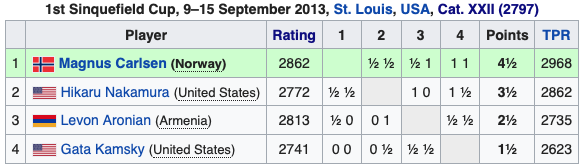
\includegraphics[width=0.75\textwidth]{figures/SinquefieldCup2013}
\end{figure}
\vfill
Note the uniform distribution of total points for each player, this data is very rankable.
\end{frame}

\begin{frame}{Remarks}
The next most rankable year is 2014.
The scorecard for that year is shown below.
\vfill
\begin{figure}[H]
\centering
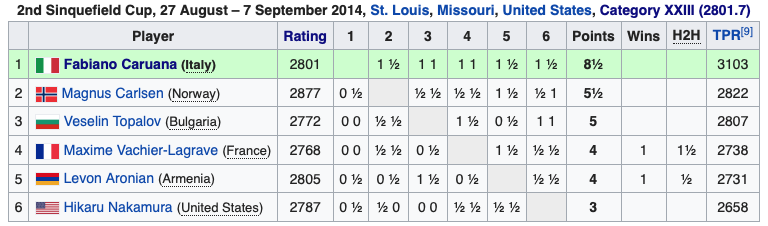
\includegraphics[width=0.75\textwidth]{figures/SinquefieldCup2014}
\end{figure}
\vfill
Note that this is the year that Fabiano went on his historical run.
However, there is a tie between 4 and 5 and not much difference between 2 and 3; hence, this year is slightly less rankable than 2013.
\end{frame}

\begin{frame}{Remarks}
The least rankable years were 2016 and 2018. 
Both scorecards are shown below.
\vfill
\begin{figure}[H]
\centering
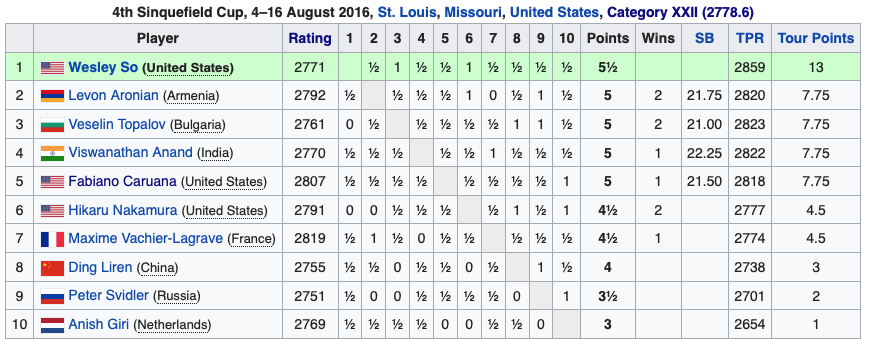
\includegraphics[width=0.75\textwidth]{figures/SinquefieldCup2016} \\
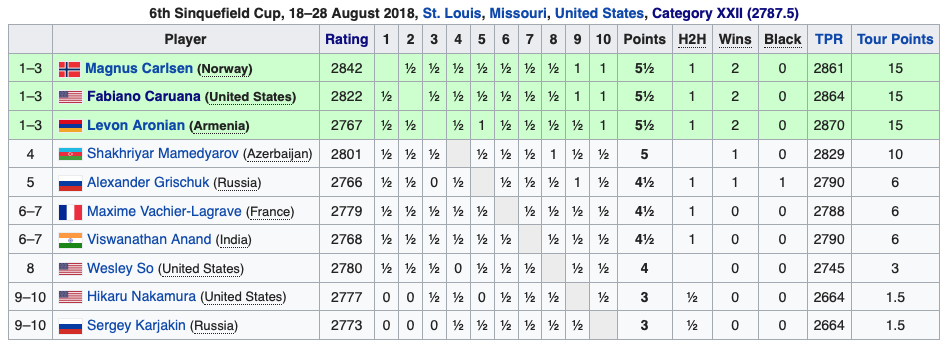
\includegraphics[width=0.75\textwidth]{figures/SinquefieldCup2018}
\end{figure}
\end{frame}

\begin{frame}{Remarks}
\begin{itemize}
\item	There is a 4 way tie for second place in 2016.
	 Furthermore, each place is only separated by half a point.
\vfill
\item Similarly, in 2018 there was a 3 way tie for first place. 
	Interestingly, the winners agreed to split the prize and not deal with elimination games.
\vfill
\item	Certainly, these years are less rankable than 2013 and 2014.
\end{itemize}
\end{frame}

%%%%%%%%%%%%%%%%%%%%%%%%%%%%%%%%%%%%%%%%%%%%%%%%%%%%%%
%								The Ranking Fit
%%%%%%%%%%%%%%%%%%%%%%%%%%%%%%%%%%%%%%%%%%%%%%%%%%%%%%
\section{The Ranking Fit}

\begin{frame}{Definition}
The ranking fit refers to how well a ranking ``fits" or ``matches" the data from a certain system.
\vfill
We measure the ranking fit based on the number of changes made to the ranking when new data from a system is considered.
\end{frame}

\begin{frame}{Sinquefield Cup Ranking Fit}
\begin{itemize}
\item	We rate the players in the tournament based on their ``local" Elo rating, where each player starts at zero and is updated based on their performance in that round.
\vfill
\item	We rank the players in the tournament by their local Elo rating.
\vfill
\item Let $k$ denote the number of changes in our ranking from the previous round, and let $n$ denote the total number of players in the tournament.
	Then, the ranking fit is defined by
	\[
	1 - \frac{k}{n}.
	\] 
\end{itemize}
\end{frame}

\begin{frame}{Round by Round Ranking Fit}
\centering
\resizebox{0.9\textwidth}{!}{% Line Plot
\begin{tikzpicture}
	\begin{axis}[
		xlabel = Round Number,
		ylabel =  Ranking Fit,
		legend pos = outer north east,
		cycle list name = color]
		\addplot coordinates{
			(1,0)
			(2,0.5)
			(3,1)
			(4,0.5)
			(5,1)
			(6,1)
		};
		\addplot coordinates{
			(1,0)
			(2,0.3333)
			(3,0.1667)
			(4,0.5)
			(5,0.1667)
			(6,0.6667)
			(7,0.6667)
			(8,1)
			(9,1)
			(10,0.6667)
		};
		\addplot coordinates{
			(1,0)
			(2,0)
			(3,0.3)
			(4,0.4)
			(5,0.2)
			(6,0.3)
			(7,0.3)
			(8,0.8)
			(9,0.6)
		};
		\addplot coordinates{
			(1,0)
			(2,0)
			(3,0.5)
			(4,0.8)
			(5,0.3)
			(6,0.2)
			(7,0.8)
			(8,0.1)
			(9,0.4)
		};
		\addplot coordinates{
			(1,0)
			(2,0.2)
			(3,0.8)
			(4,0.3)
			(5,0.1)
			(6,0.7)
			(7,0.6)
			(8,0.8)
			(9,0.2)
		};
		\addplot coordinates{
			(1,0)
			(2,0.3)
			(3,0.6)
			(4,0.5)
			(5,0.6)
			(6,0.5)
			(7,0.6)
			(8,1)
			(9,0.1)
		};
		\legend{Year 2013, Year 2014,Year 2015, Year 2016, Year 2017, Year 2018}
	\end{axis}
\end{tikzpicture}%
}
\end{frame}

\begin{frame}{Remarks}
\begin{itemize}
\item	Something very exciting happened in the last round of 2018; indeed, only one player had the same ranking in round 9 as they did in round 8.
\vfill
\item	If you compare the last round Ranking Fit and the last round Rankability, the correlation is $0.83$. 
\vfill
\item	Ranking Fit seems (to me) very related to predictability. 
\end{itemize}
\end{frame}

\end{document}